\documentclass{standalone}
\usepackage{tikz}
\usetikzlibrary{patterns, positioning}


\begin{document}
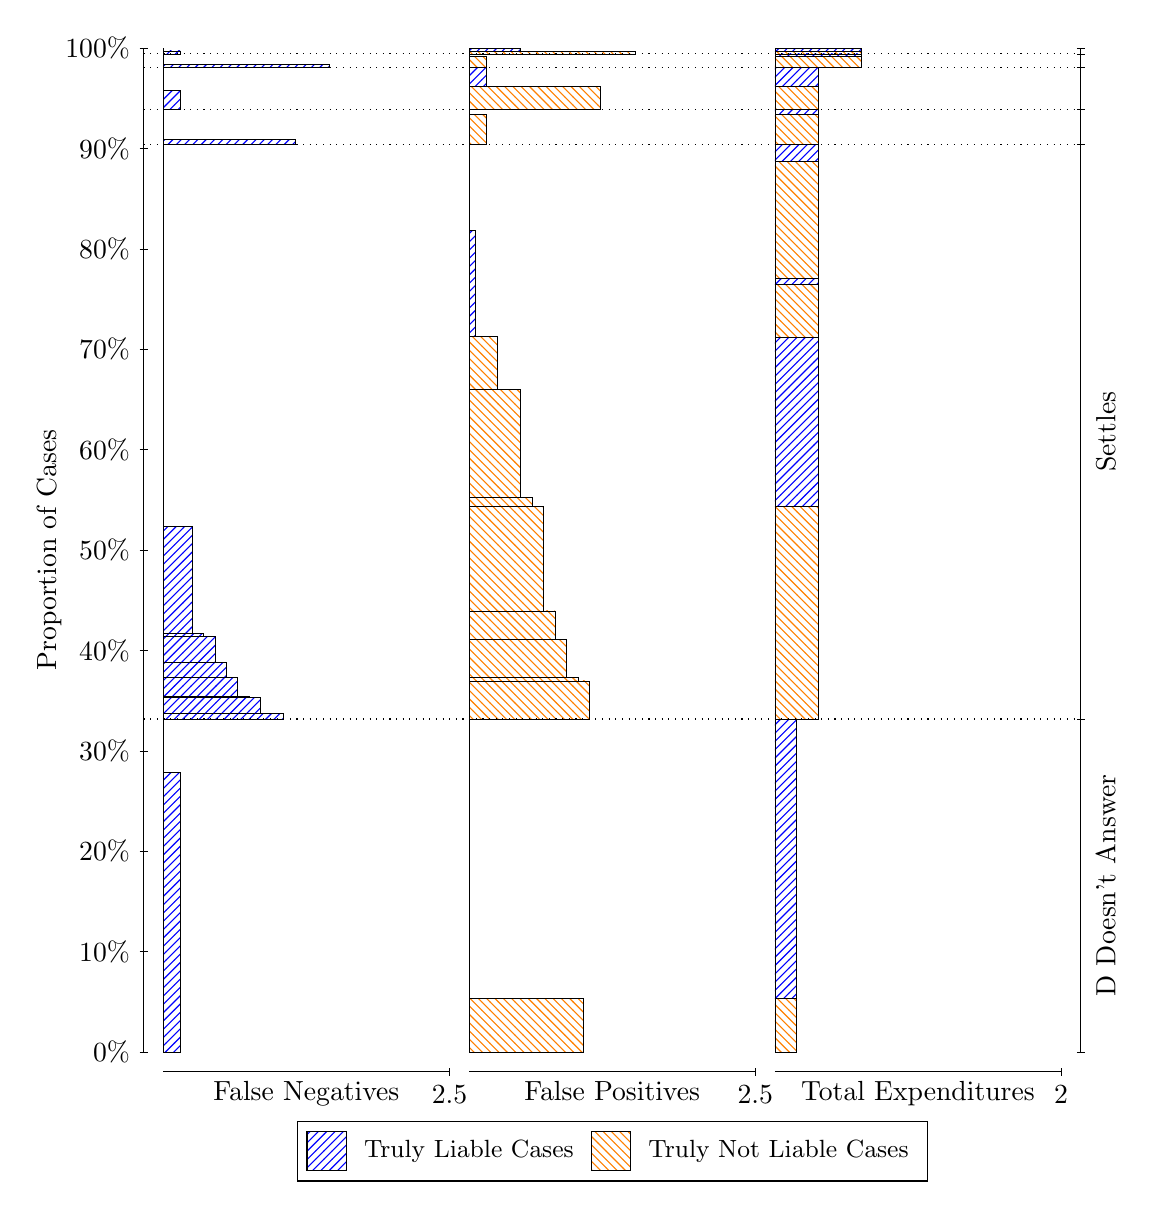
\begin{tikzpicture}
\draw[black, very thin] (1.5,1.75) -- (1.5,14.5);
\node[rotate=90, text=black, anchor=center] at (0.3, 8.125) {Proportion of Cases};
\draw[black, very thin] (1.45,1.75) -- (1.55,1.75);
\node[text=black, anchor=east] at (1.45, 1.75) {0\%};
\draw[black, very thin] (1.45,3.025) -- (1.55,3.025);
\node[text=black, anchor=east] at (1.45, 3.025) {10\%};
\draw[black, very thin] (1.45,4.3) -- (1.55,4.3);
\node[text=black, anchor=east] at (1.45, 4.3) {20\%};
\draw[black, very thin] (1.45,5.575) -- (1.55,5.575);
\node[text=black, anchor=east] at (1.45, 5.575) {30\%};
\draw[black, very thin] (1.45,6.85) -- (1.55,6.85);
\node[text=black, anchor=east] at (1.45, 6.85) {40\%};
\draw[black, very thin] (1.45,8.125) -- (1.55,8.125);
\node[text=black, anchor=east] at (1.45, 8.125) {50\%};
\draw[black, very thin] (1.45,9.4) -- (1.55,9.4);
\node[text=black, anchor=east] at (1.45, 9.4) {60\%};
\draw[black, very thin] (1.45,10.675) -- (1.55,10.675);
\node[text=black, anchor=east] at (1.45, 10.675) {70\%};
\draw[black, very thin] (1.45,11.95) -- (1.55,11.95);
\node[text=black, anchor=east] at (1.45, 11.95) {80\%};
\draw[black, very thin] (1.45,13.225) -- (1.55,13.225);
\node[text=black, anchor=east] at (1.45, 13.225) {90\%};
\draw[black, very thin] (1.45,14.5) -- (1.55,14.5);
\node[text=black, anchor=east] at (1.45, 14.5) {100\%};

\draw[black, very thin] (13.4,1.75) -- (13.4,14.5);
\draw[black, very thin] (13.35,1.75) -- (13.45,1.75);
\node[anchor=west] at (13.35, 1.75) {};
\draw[black, very thin] (13.35,5.9783) -- (13.45,5.9783);
\node[anchor=west] at (13.35, 5.9783) {};
\draw[black, very thin] (13.35,13.278) -- (13.45,13.278);
\node[anchor=west] at (13.35, 13.278) {};
\draw[black, very thin] (13.35,13.718) -- (13.45,13.718);
\node[anchor=west] at (13.35, 13.718) {};
\draw[black, very thin] (13.35,14.255) -- (13.45,14.255);
\node[anchor=west] at (13.35, 14.255) {};
\draw[black, very thin] (13.35,14.426) -- (13.45,14.426);
\node[anchor=west] at (13.35, 14.426) {};
\draw[black, very thin] (13.35,14.5) -- (13.45,14.5);
\node[anchor=west] at (13.35, 14.5) {};

\draw[black, very thin, pattern color=blue, pattern=north east lines] (1.75,1.75) rectangle (1.968,5.3005);
\draw[black, very thin, pattern color=orange, pattern=north west lines] (1.75,5.3005) rectangle (1.75,5.9783);
\draw[black, very thin, pattern color=blue, pattern=north east lines] (1.75,5.9783) rectangle (3.276,6.0533);
\draw[black, very thin, pattern color=blue, pattern=north east lines] (1.75,6.0533) rectangle (2.9853,6.2513);
\draw[black, very thin, pattern color=blue, pattern=north east lines] (1.75,6.2513) rectangle (2.84,6.2686);
\draw[black, very thin, pattern color=blue, pattern=north east lines] (1.75,6.2686) rectangle (2.6947,6.5097);
\draw[black, very thin, pattern color=blue, pattern=north east lines] (1.75,6.5097) rectangle (2.5493,6.7009);
\draw[black, very thin, pattern color=blue, pattern=north east lines] (1.75,6.7009) rectangle (2.404,7.0245);
\draw[black, very thin, pattern color=blue, pattern=north east lines] (1.75,7.0245) rectangle (2.2587,7.0708);
\draw[black, very thin, pattern color=blue, pattern=north east lines] (1.75,7.0708) rectangle (2.1133,8.4206);
\draw[black, very thin, pattern color=orange, pattern=north west lines] (1.75,8.4206) rectangle (1.75,13.278);
\draw[black, very thin, pattern color=blue, pattern=north east lines] (1.75,13.278) rectangle (3.4213,13.342);
\draw[black, very thin, pattern color=orange, pattern=north west lines] (1.75,13.342) rectangle (1.75,13.718);
\draw[black, very thin, pattern color=blue, pattern=north east lines] (1.75,13.718) rectangle (1.968,13.962);
\draw[black, very thin, pattern color=orange, pattern=north west lines] (1.75,13.962) rectangle (1.75,14.255);
\draw[black, very thin, pattern color=blue, pattern=north east lines] (1.75,14.255) rectangle (3.8573,14.291);
\draw[black, very thin, pattern color=orange, pattern=north west lines] (1.75,14.291) rectangle (1.75,14.426);
\draw[black, very thin, pattern color=blue, pattern=north east lines] (1.75,14.426) rectangle (1.968,14.464);
\draw[black, very thin, pattern color=orange, pattern=north west lines] (1.75,14.464) rectangle (1.75,14.5);
\draw[black, very thin, pattern color=orange, pattern=north west lines] (5.6333,1.75) rectangle (7.0867,2.4279);
\draw[black, very thin, pattern color=blue, pattern=north east lines] (5.6333,2.4279) rectangle (5.6333,5.9783);
\draw[black, very thin, pattern color=orange, pattern=north west lines] (5.6333,5.9783) rectangle (7.1593,6.4615);
\draw[black, very thin, pattern color=orange, pattern=north west lines] (5.6333,6.4615) rectangle (7.014,6.5114);
\draw[black, very thin, pattern color=orange, pattern=north west lines] (5.6333,6.5114) rectangle (6.8687,6.9939);
\draw[black, very thin, pattern color=orange, pattern=north west lines] (5.6333,6.9939) rectangle (6.7233,7.3504);
\draw[black, very thin, pattern color=orange, pattern=north west lines] (5.6333,7.3504) rectangle (6.578,8.6783);
\draw[black, very thin, pattern color=orange, pattern=north west lines] (5.6333,8.6783) rectangle (6.4327,8.79);
\draw[black, very thin, pattern color=orange, pattern=north west lines] (5.6333,8.79) rectangle (6.2873,10.163);
\draw[black, very thin, pattern color=orange, pattern=north west lines] (5.6333,10.163) rectangle (5.9967,10.836);
\draw[black, very thin, pattern color=blue, pattern=north east lines] (5.6333,10.836) rectangle (5.706,12.186);
\draw[black, very thin, pattern color=blue, pattern=north east lines] (5.6333,12.186) rectangle (5.6333,13.278);
\draw[black, very thin, pattern color=orange, pattern=north west lines] (5.6333,13.278) rectangle (5.8513,13.654);
\draw[black, very thin, pattern color=blue, pattern=north east lines] (5.6333,13.654) rectangle (5.6333,13.718);
\draw[black, very thin, pattern color=orange, pattern=north west lines] (5.6333,13.718) rectangle (7.3047,14.01);
\draw[black, very thin, pattern color=blue, pattern=north east lines] (5.6333,14.01) rectangle (5.8513,14.255);
\draw[black, very thin, pattern color=orange, pattern=north west lines] (5.6333,14.255) rectangle (5.8513,14.39);
\draw[black, very thin, pattern color=blue, pattern=north east lines] (5.6333,14.39) rectangle (5.6333,14.426);
\draw[black, very thin, pattern color=orange, pattern=north west lines] (5.6333,14.426) rectangle (7.7407,14.462);
\draw[black, very thin, pattern color=blue, pattern=north east lines] (5.6333,14.462) rectangle (6.2873,14.5);
\draw[black, very thin, pattern color=orange, pattern=north west lines] (9.5167,1.75) rectangle (9.7892,2.4279);
\draw[black, very thin, pattern color=blue, pattern=north east lines] (9.5167,2.4279) rectangle (9.7892,5.9783);
\draw[black, very thin, pattern color=orange, pattern=north west lines] (9.5167,5.9783) rectangle (10.062,8.6783);
\draw[black, very thin, pattern color=blue, pattern=north east lines] (9.5167,8.6783) rectangle (10.062,10.83);
\draw[black, very thin, pattern color=orange, pattern=north west lines] (9.5167,10.83) rectangle (10.062,11.503);
\draw[black, very thin, pattern color=blue, pattern=north east lines] (9.5167,11.503) rectangle (10.062,11.578);
\draw[black, very thin, pattern color=orange, pattern=north west lines] (9.5167,11.578) rectangle (10.062,13.063);
\draw[black, very thin, pattern color=blue, pattern=north east lines] (9.5167,13.063) rectangle (10.062,13.278);
\draw[black, very thin, pattern color=orange, pattern=north west lines] (9.5167,13.278) rectangle (10.062,13.654);
\draw[black, very thin, pattern color=blue, pattern=north east lines] (9.5167,13.654) rectangle (10.062,13.718);
\draw[black, very thin, pattern color=orange, pattern=north west lines] (9.5167,13.718) rectangle (10.062,14.01);
\draw[black, very thin, pattern color=blue, pattern=north east lines] (9.5167,14.01) rectangle (10.062,14.255);
\draw[black, very thin, pattern color=orange, pattern=north west lines] (9.5167,14.255) rectangle (10.607,14.39);
\draw[black, very thin, pattern color=blue, pattern=north east lines] (9.5167,14.39) rectangle (10.607,14.426);
\draw[black, very thin, pattern color=orange, pattern=north west lines] (9.5167,14.426) rectangle (10.607,14.462);
\draw[black, very thin, pattern color=blue, pattern=north east lines] (9.5167,14.462) rectangle (10.607,14.5);
\draw[black, dotted] (1.5,5.9783) -- (13.4,5.9783);
\draw[black, dotted] (1.5,13.278) -- (13.4,13.278);
\draw[black, dotted] (1.5,13.718) -- (13.4,13.718);
\draw[black, dotted] (1.5,14.255) -- (13.4,14.255);
\draw[black, dotted] (1.5,14.426) -- (13.4,14.426);
\draw[black, very thin] (1.75,1.5) -- (5.3833,1.5);
\node[text=black, anchor=north] at (3.5667, 1.5) {False Negatives};
\draw[black, very thin] (5.3833,1.45) -- (5.3833,1.55);
\node[text=black, anchor=north] at (5.3833, 1.45) {2.5};

\draw[black, very thin] (5.6333,1.5) -- (9.2667,1.5);
\node[text=black, anchor=north] at (7.45, 1.5) {False Positives};
\draw[black, very thin] (9.2667,1.45) -- (9.2667,1.55);
\node[text=black, anchor=north] at (9.2667, 1.45) {2.5};

\draw[black, very thin] (9.5167,1.5) -- (13.15,1.5);
\node[text=black, anchor=north] at (11.333, 1.5) {Total Expenditures};
\draw[black, very thin] (13.15,1.45) -- (13.15,1.55);
\node[text=black, anchor=north] at (13.15, 1.45) {2};

\node[text=black, centered, rotate=90] at (13.72, 3.8642) {D Doesn't Answer};
\node[text=black, centered, rotate=90] at (13.72, 9.6282) {Settles};





\draw (7.449999999999999,1.5) node[draw=none] (baseCoordinate) {};
\begin{scope}[align=center]
        \matrix[scale=0.5, draw=black, below=0.5cm of baseCoordinate, nodes={draw}, column sep=0.1cm]{
            \node[rectangle, draw, minimum width=0.5cm, minimum height=0.5cm, pattern color=blue, pattern=north east lines] {}; &
            \node[draw=none, font=\small, text=black] (B) {Truly Liable Cases}; &
            \node[rectangle, draw, minimum width=0.5cm, minimum height=0.5cm, pattern color=orange, pattern=north west lines] {}; &
            \node[draw=none, font=\small, text=black] (B) {Truly Not Liable Cases}; \\
            };
\end{scope}

\end{tikzpicture}
\end{document}